\section{Pengembangan Prototipe \textit{High-Fidelity} Iterasi Kedua}
\label{sec:hifi_2}

Menurut hasil pengujian pada prototipe \textit{high-fidelity} iterasi pertama, solusi desain masih banyak ruang untuk ditingkatkan kualitasnya. Maka dari itu ditentukan bahwa perlu dirancang prototipe \textit{high-fidelity} iterasi kedua. Pada iterasi ini, prototipe akan memuat hasil implementasi perbaikan-perbaikan berdasarkan daftar rencana perbaikan pada Tabel \ref{tab:daftar_perbaikan_hifi}.

% \subsection{Implementasi Prototipe \textit{High-Fidelity} }
% \label{subsec:hifi_2_implementasi}

Berikut adalah perbaikan yang dilakukan dalam implementasi prototipe \textit{high-fidelity} iterasi kedua.

\begin{enumerate}
  \item \textbf{PH-01}: Mengatur opsi default pada Bedtime Mode menjadi Based on schedule
  \subitem Hal ini mengacu pada prinsip desain \textit{Empowerment} (DP-01), di mana opsi sebuah pengaturan sebaiknya memiliki opsi \textit{default} yang membantu pengguna memperbaiki perilakunya. Pada perbaikan, Bedtime Mode akan secara \textit{default} terpasang sebagai Based on schedule ketika pengguna pertama kali masuk ke halamannya. Hasil perbaikan dapat dilihat pada Gambar \ref{img:perbaikan_1}.
  
  \begin{figure}[h]
    \centering
    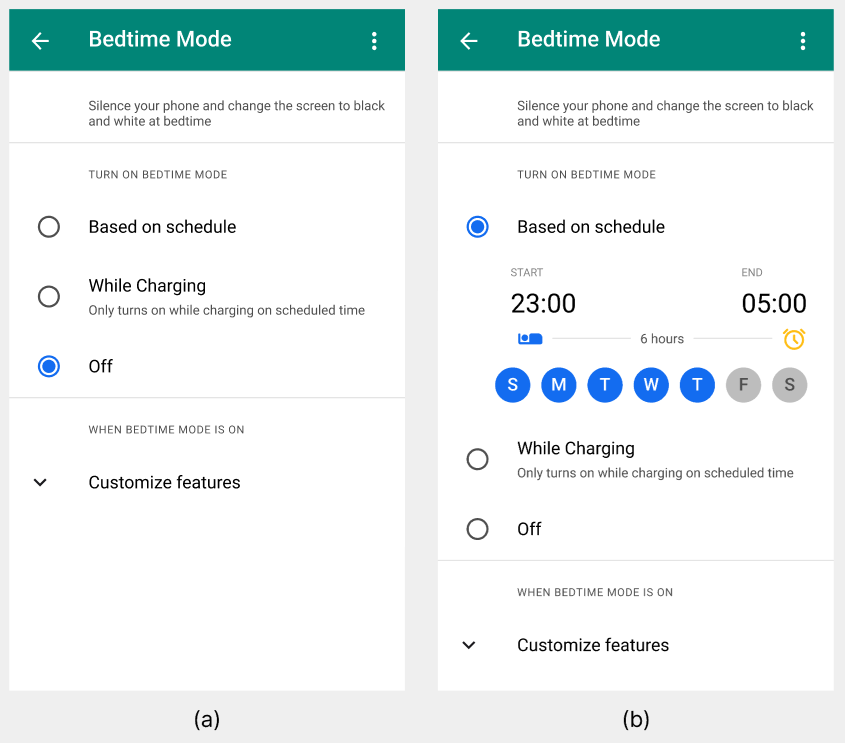
\includegraphics[width=0.6\textwidth]{hifi2/perbaikan_1.png}
    \caption{Halaman Bedtime Mode saat pertama kali dinavigasi, sebelum (a) dan setelah perbaikan (b)}
    \label{img:perbaikan_1}
  \end{figure}
  \FloatBarrier

  
  \item \textbf{PH-02}: Mempertahankan desain \textit{widget} Dashboard
  \subitem Keputusan mengenai keluhan seorang pengguna mengenai terbatasnya fungsionalitas dari \textit{widget} Dashboard (W-01) ini ditentukan karena mengacu pada sifat sebuah \textit{widget} aplikasi yaitu sebagai tampilan sederhana yang memuat fungsionalitas paling penting dari sebuah aplikasi. Maka dari itu, desain dari \textit{widget} Dashboard ditentukan sudah final. Jika pengguna ingin melihat informasi lebih tentang penggunaan aplikasi / \textit{smartphone}, maka pengguna dapat langsung menavigasi ke halaman Dashboard (H-02) dengan menekan \textit{widget} Dashboard.  

  \item \textbf{PH-03}: Menghapus navigasi dari halaman Dashboard ke halaman Pengaturan Jadwal App Timer, tanpa menghapus indikator App Timer
  \subitem Indikator App Timer yang terletak di item daftar aplikasi pada halaman Dashboard (H-2) berguna juga sebagai navigasi ke halaman Pengaturan Jadwal App Timer (H-10). Hal ini dinilai membingungkan ketika seorang pengguna hanya ingin melihat ringkasan penggunaan aplikasinya. Maka dari itu, navigasi ke halaman Pengaturan Jadwal App Timer lewat indikator ini dihapus, tanpa menghapus indikator dari App Timer untuk aplikasinya. Untuk mengatur App Timer sebuah aplikasi, pengguna dapat melakukan navigasi lewat halaman App Timer (H-03) atau halaman Ringkasan Penggunaan Aplikasi (H-07).

  \item \textbf{PH-04}: Menambahkan pesan pengingat untuk aksi yang cukup kritis seperti mematikan Focus Mode atau App Timer
  \subitem Keputusan ini diambil berdasarkan prinsip desain \textit{Feedback} (DP-06), di mana sebuah aksi layaknya dipasangi dengan sebuah reaksi untuk memastikan apakah pengguna yakin ingin melakukan aksinya atau tidak. Prinsip desain \textit{Feedback} sering dipadukan dengan aksi-aksi yang bersifat kritis, dalam hal ini mematikan jadwal App Timer atau Focus Mode. Hal ini juga berkaitan dengan \textit{usability goal Safety}, di mana sebuah aplikasi harus memberikan rasa aman kepada penggunanya terutama dalam melakukan aksi-aksi yang kritis, salah satu caranya dengan mencegah kesalahan.
  \subitem Maka dari itu, sebagai perbaikan prototipe ketika pengguna menekan tombol "Turn off for today" pada fitur App Timer atau Focus Mode, pengguna akan disambut dengan pesan konfirmasi apakah aksinya benar ingin dilakukan atau tidak. Tampilan pesan konfirmasi dapat dilihat pada Gambar \ref{img:perbaikan_4}.

  \begin{figure}[h]
    \centering
    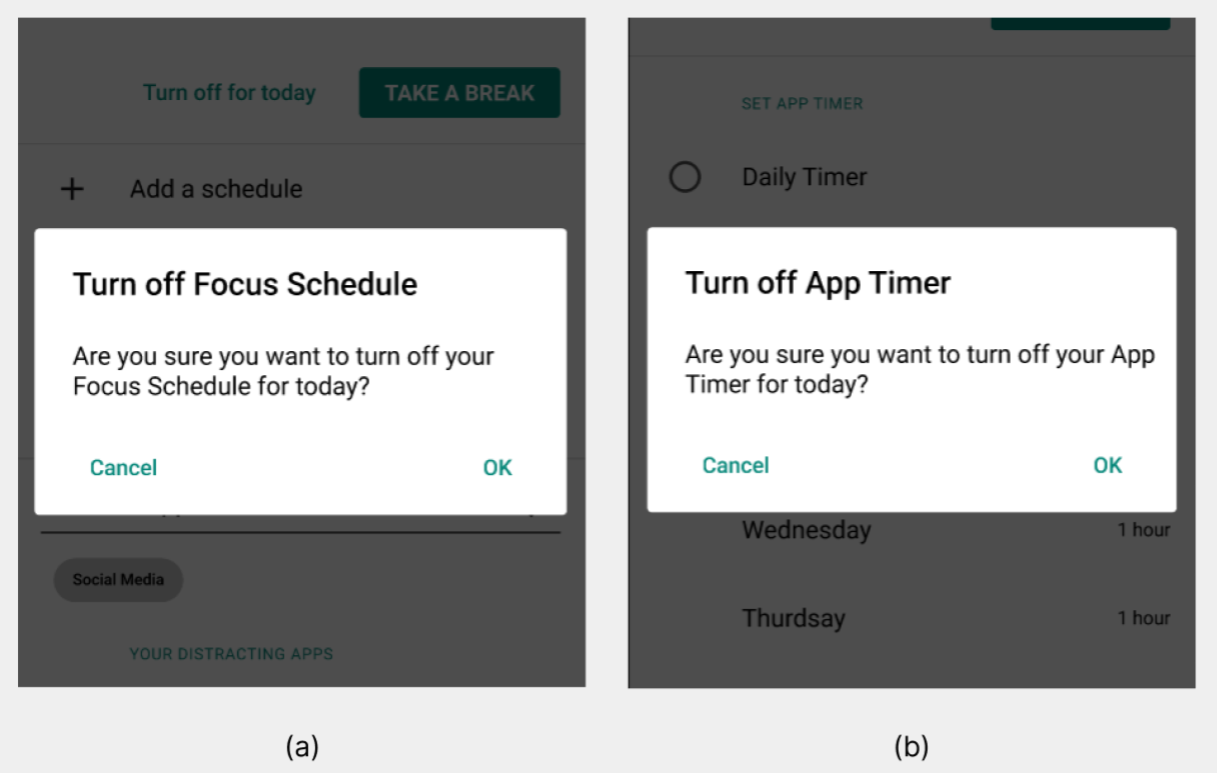
\includegraphics[width=0.6\textwidth]{hifi2/perbaikan_4.png}
    \caption{Pesan konfirmasi saat menekan tombol "Turn off for today" pada fitur Focus Mode (a) dan fitur App Timer (b)}
    \label{img:perbaikan_4}
  \end{figure}
  \FloatBarrier

  \item \textbf{PH-05}: Menunda memunculkan evaluasi tepat setelah menentukan Daily Goal 
  \subitem Terdapat pengguna yang mengeluhkan bahwa evaluasi terhadap Daily Goal yang langsung dimunculkan sesaat setelah memasang Daily Goal cukup membingungkan. Maka dari itu, pengguna akan diberitahukan bahwa evaluasi untuk Daily Goal dapat dilakukan di akhir hari, sesuai dengan jadwal fitur Smartphone Usage Evaluation yang ditentukan atau hingga pengguna kembali ke halaman Daily Goal. Pesan yang dimunculkan dirancang sesuai dengan pedoman dari prinsip desain \textit{Feedback} (DP-06). Perbandingan hasil perbaikan dengan tampilan sebelumnya dapat dilihat pada Gambar \ref{img:perbaikan_5}.

  \begin{figure}[h]
    \centering
    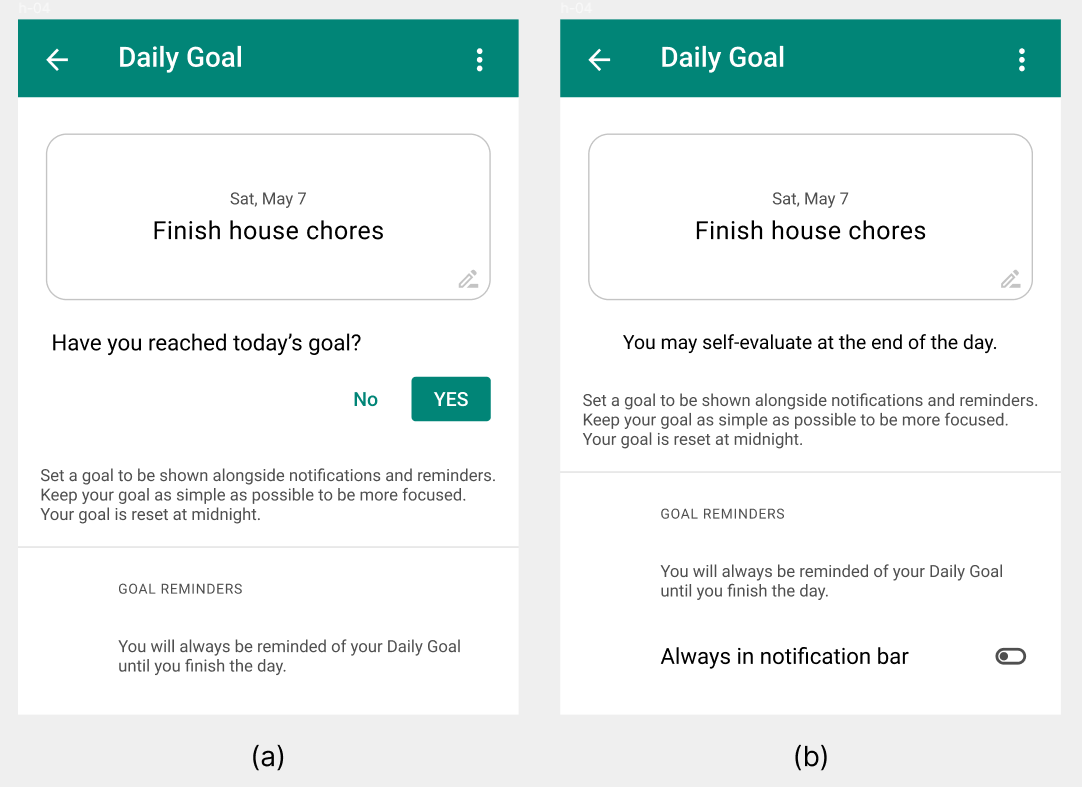
\includegraphics[width=0.6\textwidth]{hifi2/perbaikan_5.png}
    \caption{Tampilan halaman Daily Goal sesaat setelah menentukan Daily Goal, sebelum (a) dan sesudah perbaikan (b)}
    \label{img:perbaikan_5}
  \end{figure}
  \FloatBarrier
  
  \item \textbf{PH-06}: Memindahkan fitur Smartphone Usage Evaluation dari halaman Daily Goal ke halaman baru
  \subitem Pada saat pengujian ditemukan beberapa partisipan yang kebingungan mencari fitur Smartphone Usage Evaluation dan mereka berpendapat bahwa penempatan fitur ini di halaman Daily Goal kurang tepat. Maka dari itu, perlu dibuat sebuah halaman baru, halaman Daily Usage Evaluation, untuk menampung fitur Smartphone Usage Evaluation yang dapat diakses lewat halaman Main Menu (H-01). Perbaikan tampilan untuk halaman Daily Goal dapat dilihat pada Gambar \ref{img:perbaikan_6-1}, sedangkan halaman baru beserta tombol navigasi untuk fitur Smartphone Usage Evaluation dapat dilihat pada Gambar \ref{img:perbaikan_6-2}.
  
  \begin{figure}[h]
    \centering
    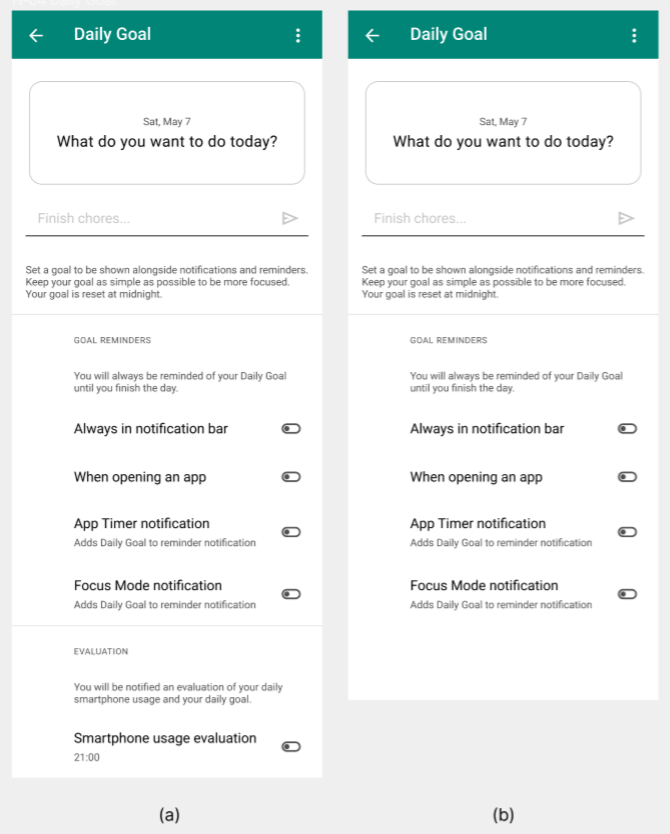
\includegraphics[width=0.55\textwidth]{hifi2/perbaikan_6-1.png}
    \caption{Tampilan halaman Daily Goal sebelum (a) dan sesudah perbaikan (b)}
    \label{img:perbaikan_6-1}
  \end{figure}
  \FloatBarrier
  
  \begin{figure}[h]
    \centering
    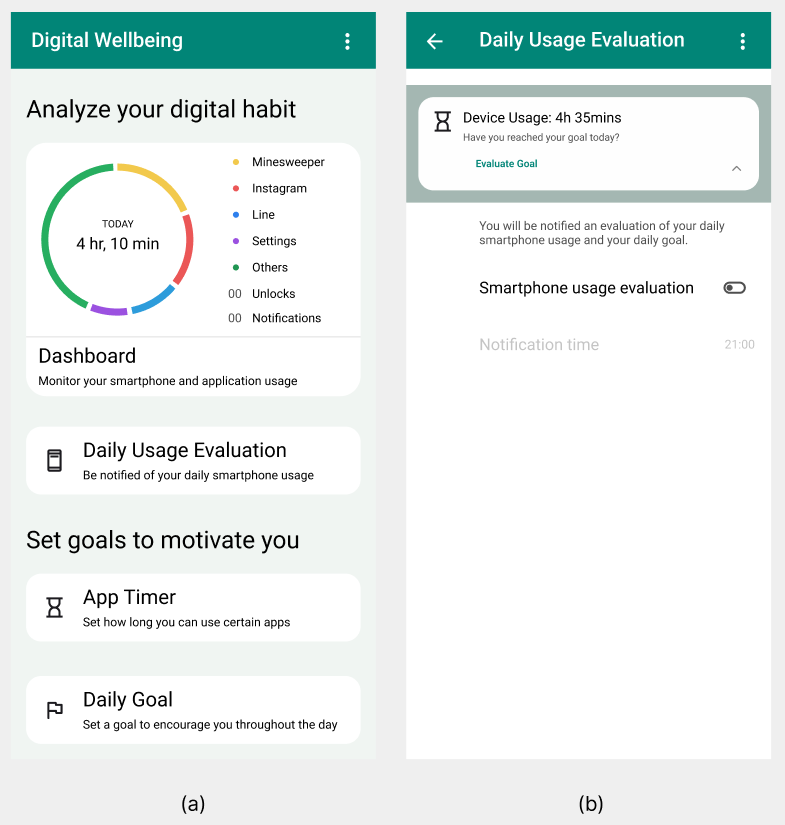
\includegraphics[width=0.55\textwidth]{hifi2/perbaikan_6-2.png}
    \caption{Tampilan halaman Main Menu setelah perbaikan (a) dan tampilan halaman baru untuk fitur Smartphone Usage Evaluation (b)}
    \label{img:perbaikan_6-2}
  \end{figure}
  \FloatBarrier

  \item \textbf{PH-07}: Menghapus tombol penambahan App Timer dari \textit{widget} App Timer
  \subitem Terdapat pengguna yang berpendapat bahwa tombol penambahan App Timer pada \textit{widget} App Timer dinilai tidak diperlukan, karena ketika menekan tombol dan menekan bagian lain dari \textit{widget} akan menavigasi pengguna ke halaman yang sama yaitu halaman App Timer (H-03). Maka dari itu, tombol plus (+) untuk menambahkan App Timer dari \textit{widget} diputuskan untuk dihapus. Hal ini juga mempertegas tujuan dari \textit{widget} App Timer yaitu hanya untuk menampilkan daftar App Timer yang telah dipasang. Tampilan App Timer sebelum dan sesudah perbaikan dapat dilihat pada Gambar \ref{img:perbaikan_7}    

  \begin{figure}[h]
    \centering
    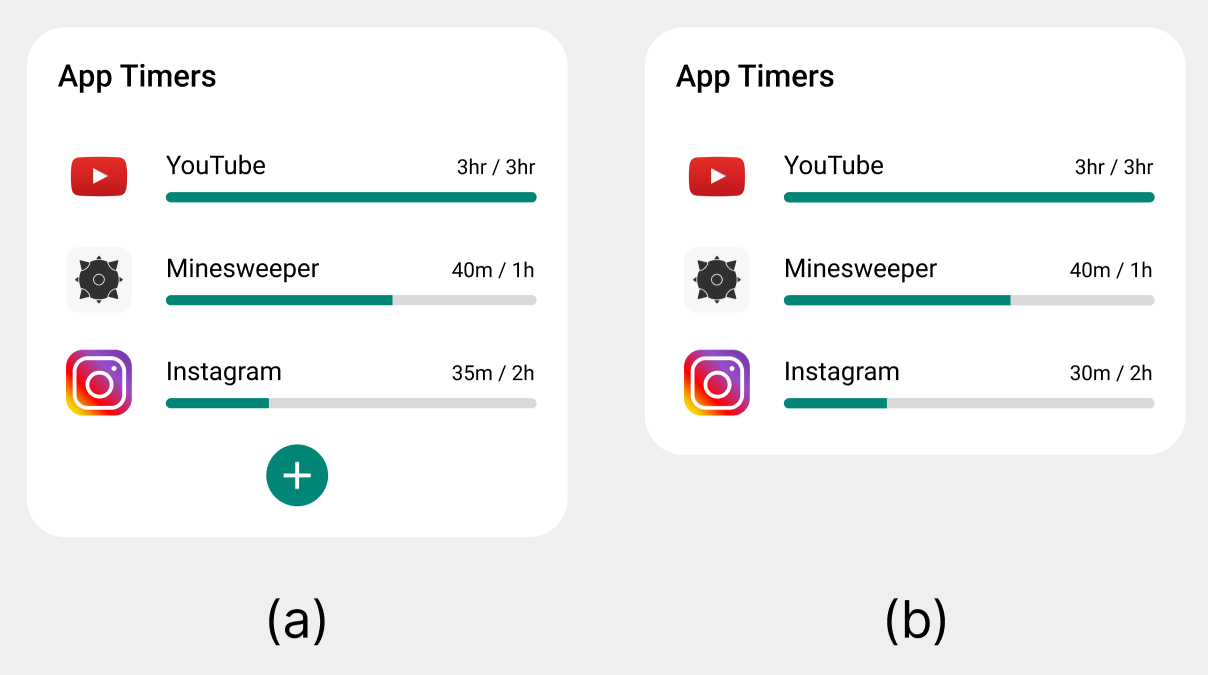
\includegraphics[width=0.6\textwidth]{hifi2/perbaikan_7.png}
    \caption{Tampilan \textit{widget} App Timer sebelum (a) dan setelah perbaikan (b)}
    \label{img:perbaikan_7}
  \end{figure}
  \FloatBarrier
  
\end{enumerate}
